%!TEX TS-program = latex
%!TEX encoding = UTF-8 Unicode

%if latexmk does not use pdflatex automatically with these lines, please use the command "latexmk -pdf" manually


\documentclass[final]{beamer}

% For more themes, color themes and font themes, see:
% http://deic.uab.es/~iblanes/beamer_gallery/index_by_theme.html
%

\mode<presentation>
{
  \usetheme{Madrid}       % or try default, Darmstadt, Warsaw, ...
  \usecolortheme{default} % or try albatross, beaver, crane, ...
  \usefonttheme{serif}    % or try default, structurebold, ...
  \setbeamertemplate{navigation symbols}{}
  \setbeamertemplate{caption}[numbered]
} 


%\usepackage{amsmath}
%\usepackage{color}
%\usepackage{pgfplots}
%\pgfplotsset{compat=1.15}

\usepackage[english]{babel}
\usepackage{hyperref}
\usepackage[T1]{fontenc}
\usepackage[utf8]{inputenc}
\usepackage{graphicx} 
\usepackage{tikz}
%\usetikzlibrary{3d}

\setlength\parindent{0pt}

\newcommand{\backupbegin}{
   \newcounter{finalframe}
   \setcounter{finalframe}{\value{framenumber}}
}
\newcommand{\backupend}{
   \setcounter{framenumber}{\value{finalframe}}
}

\def\Emax{E_{\mathrm{max}}}
\def\parton#1{\left({{#1}}\right)}
\def\parqua#1{\left[{{#1}}\right]}
\def\Ecal{{\cal E}}
\def\derp#1#2{{\partial{#1} \over \partial{#2}}}
\def\aladyn{\texttt{ALaDyn} }
\hyphenation{ex-per-i-men-tal-ly ac-cel-er-a-tion}

\title[2D-3D PIC sims and laws]{TNSA proton maximum energy laws\\for 2D and 3D PIC simulations}

\author[S.~Sinigardi]{Stefano Sinigardi}
\institute[DiFA-UniBO/INFN]{Dipartimento di Fisica e Astronomia, Universit\`a di Bologna\\INFN Sezione di Bologna\\\vspace{5mm}L3IA Collaboration\\\vspace{5mm}}

\date[26$^{th}$ September, 2017]{3$^{rd}$ EAAC Workshop \hspace{5mm} $24^{th}$-$30^{th}$ September, 2017\\\vspace{8mm}\scriptsize{IscrB-AGOS}\\Physics of Plasmas 24, 043106 (2017); doi:10.1063/1.4979901}

\begin{document}

\begin{frame}
  \titlepage
\end{frame}

%\begin{frame}
%  \tableofcontents
%\end{frame}


\section{Presentation}


%\section{Our virtual laboratory}
\begin{frame}{Our virtual laboratory}
\begin{figure}
\centering

\includegraphics[width=0.40 \textwidth]{figs/piccante_logo.png}
\hspace{1cm}
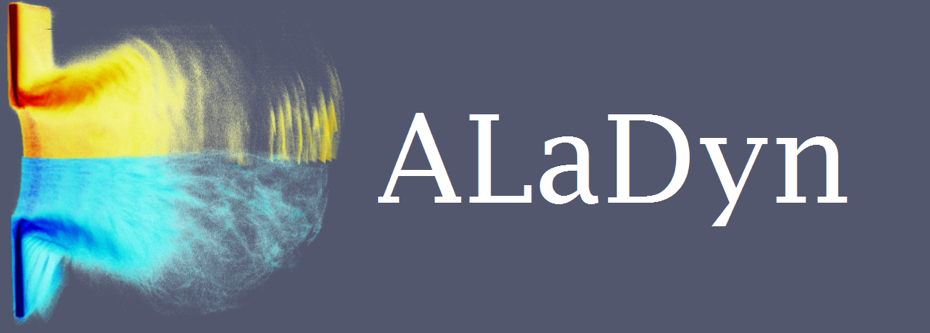
\includegraphics[width=0.40 \textwidth]{figs/ALaDyn_logo.png} 
\vspace{1cm}
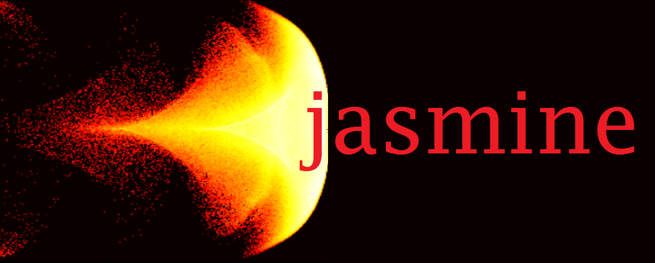
\includegraphics[width=0.40 \textwidth]{figs/jasmine_logo.png} 
\hspace{1cm}
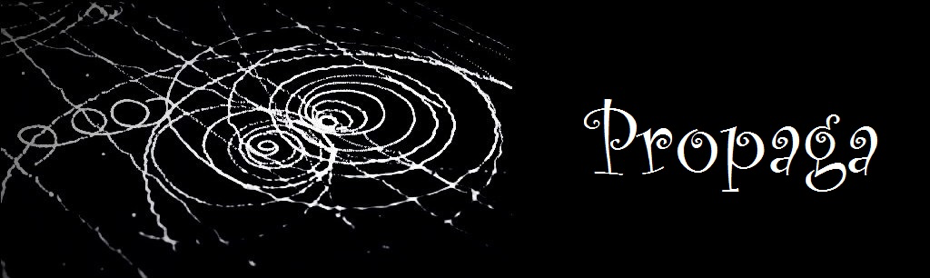
\includegraphics[width=0.40 \textwidth]{figs/Propaga_logo.png} 
\end{figure} 

\center{
Apart from jasmine, all of our codes are now free (GPL v3)

\vspace{5mm}
\href{https://github.com/ALaDyn}{webpage: https://github.com/ALaDyn}
}

\end{frame}






\begin{frame}{ALaDyn}{Recent development}
Since \aladyn became open source\footnote{we still have a version in-house a little bit different, we will release all the modules step-by-step}, almost one year ago, we released these updates:
\begin{itemize}
\item Ported \aladyn to the new Marconi HPC system deployed at CINECA (both the A1 and A2 partition)
\item Rewrote the gaseous and solid target specifications and implementations, to ease simulations for recent experiments
\item PWFA: new bunch shapes
\item Deprecated the previous toolchain, ported everything to CMake
\item Rewrote the I/O module to work around machine-level bugs on Marconi
\item Add compatibility with old-\aladyn input files
\item Usual bugfixes
\end{itemize}

\end{frame}




%\section{A consolidated regime}
%\subsection{TNSA energy spectrum from experiments and simulations}
\begin{frame}{A consolidated regime}{TNSA energy spectrum}

TNSA has a very well known energy spectrum, based on an exponential distribution with a precise cut-off energy $\Emax$ ($T$ is the proton temperature).

%\vspace{1cm}
\[
  \begin{cases}
    \displaystyle dN/dE = (\Emax/T)\,\, e^{-E/T} &\mathrm{for}\; E<\Emax \\
    \displaystyle dN/dE = 0                      &\mathrm{for}\; E>\Emax
  \end{cases}
\]
%\vspace{1cm}

\begin{figure}
\centering
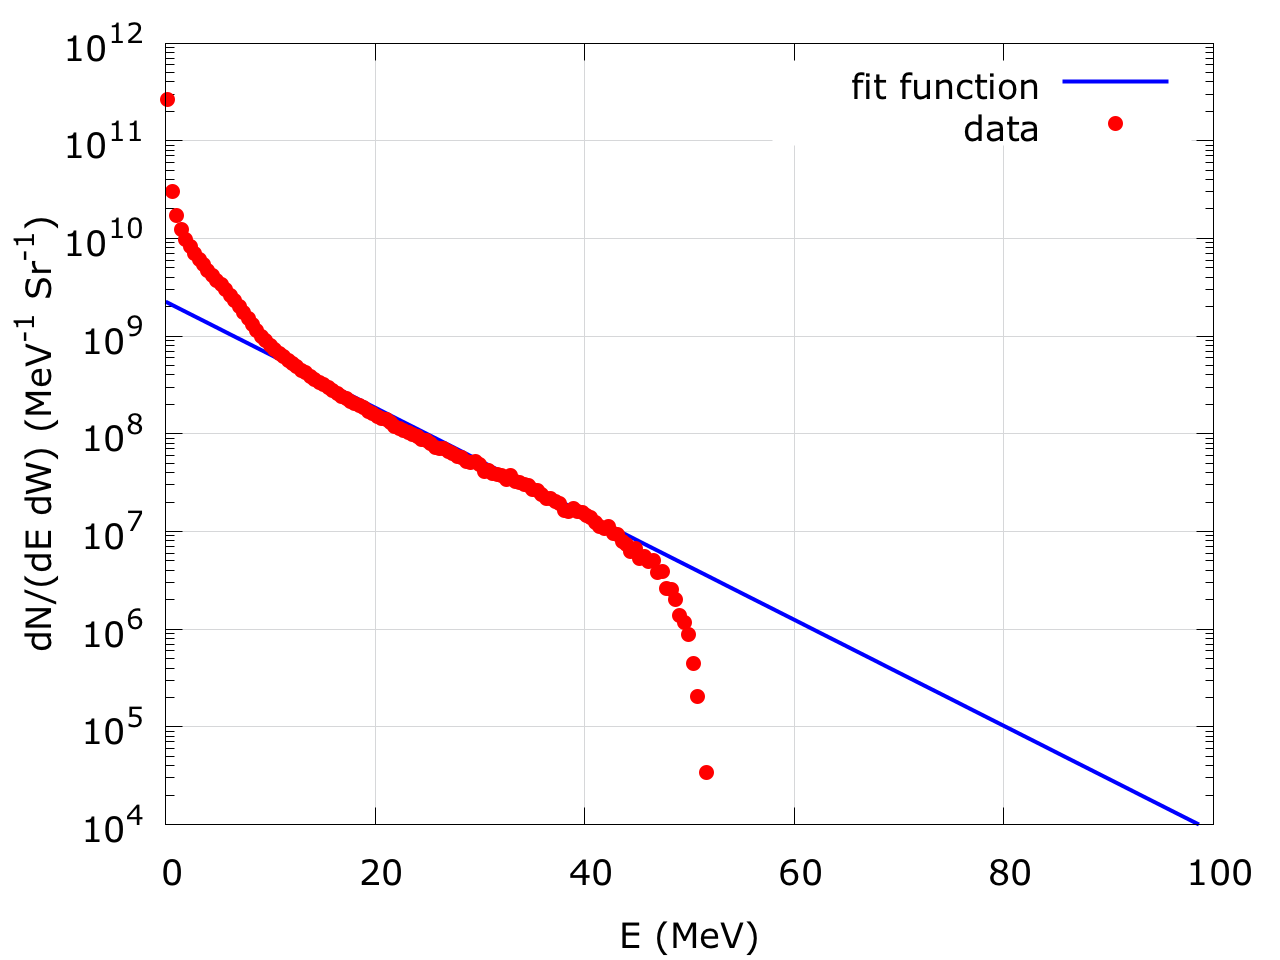
\includegraphics[width=0.40 \textwidth]{figs/Prpout12_Espec.png}
\end{figure}
% as R. Zimmermann told us the first day, 1.1 MeV was obtained with a cyclotron in ~1930

\end{frame}





%\section{Why still TNSA?}
%\subsection{INFN-L3IA experiment}
\begin{frame}{Why still TNSA?}{INFN-L3IA experiment}

\begin{itemize}
  \item laser pulse duration: $\tau=40$ fs
  \item $\lambda=0.8 \,\mu$m, P-polarized
  \item $I=2\,\cdot\,10^{19} $ W/cm$^2$, $a_0=3$
  \item waist 6.2 $\mu$m
  \item target: uniform Al foil, thickness $0.5 \mu$m $\leq L \leq 8 \mu$m
  \item contaminants: layer of H on the rear (non illuminated) side, fixed thickness $0.08 \mu$m
  \item ionization level: fixed, Al$^{9+}$, H$^{+}$
  \item electron densities: $n_e^{Al}=100 \,n_c$, $n_e^H=10\,n_c$. 
  \item neglected preplasma (the temporal contrast is assumed as infinite)
\end{itemize}

\end{frame}







%\subsection{During the acceleration mechanism }
\begin{frame}{The problem}{Numerical simulations}

\begin{figure}
\centering
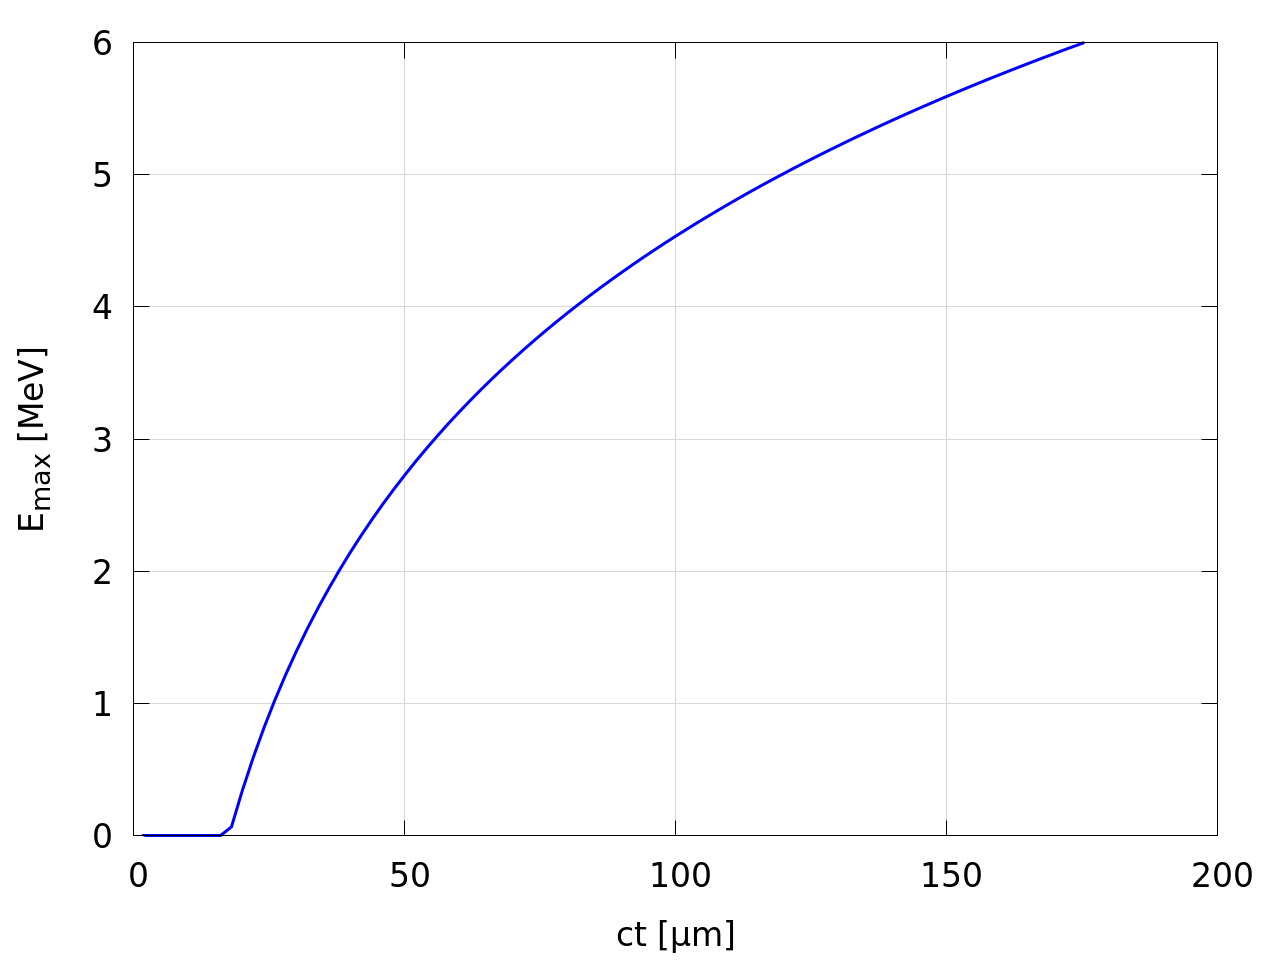
\includegraphics[width=0.40 \textwidth]{figs/problem_2d.png} 
\hspace{1cm}
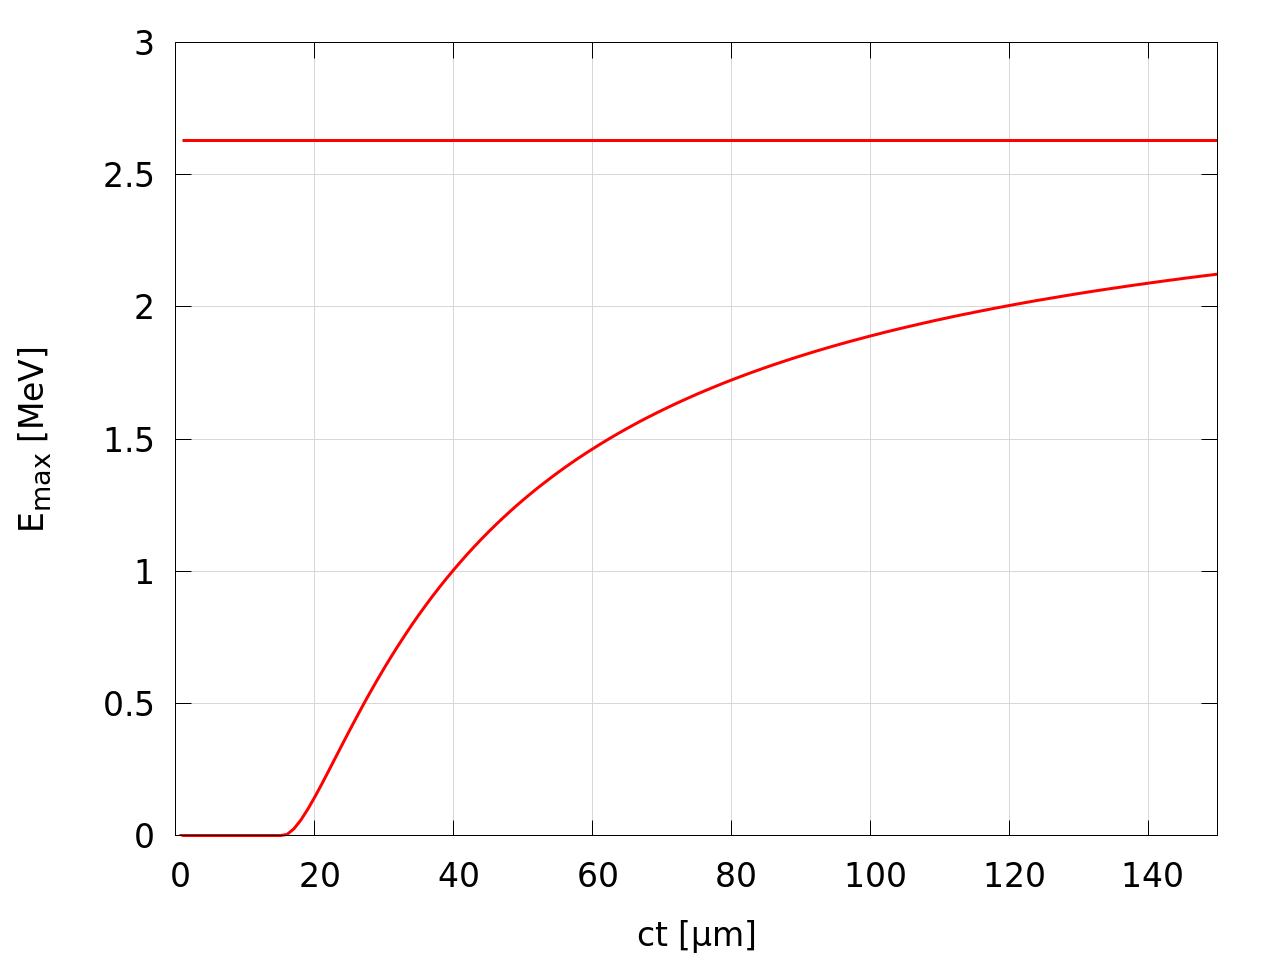
\includegraphics[width=0.40 \textwidth]{figs/problem_3d.png}
\caption{
  Maximum energy rise in time. Left: the 2D case, right: the 3D case.
}
\end{figure}


In 2D PIC TNSA simulations, a monotonic rise of $\Emax$ with time is observed whereas in 3D a slow trend towards a possible saturation to an asymptotic value is usually observed.

\end{frame}






%\section{A \textit{new simple} law to explain regime}
\begin{frame}{Two EMPIRICAL laws for $\Emax(t)$}
%We propose two empirical laws for $\Emax(t)$.
Work originated from Schreiber et al. model\footnote{Phys. Rev. Lett., 97:045005, Jul 2006}.
The acceleration of protons (contaminants) is due to the positive surface charge created on the rear target, thanks to the electron escape.

\begin{figure}
\centering
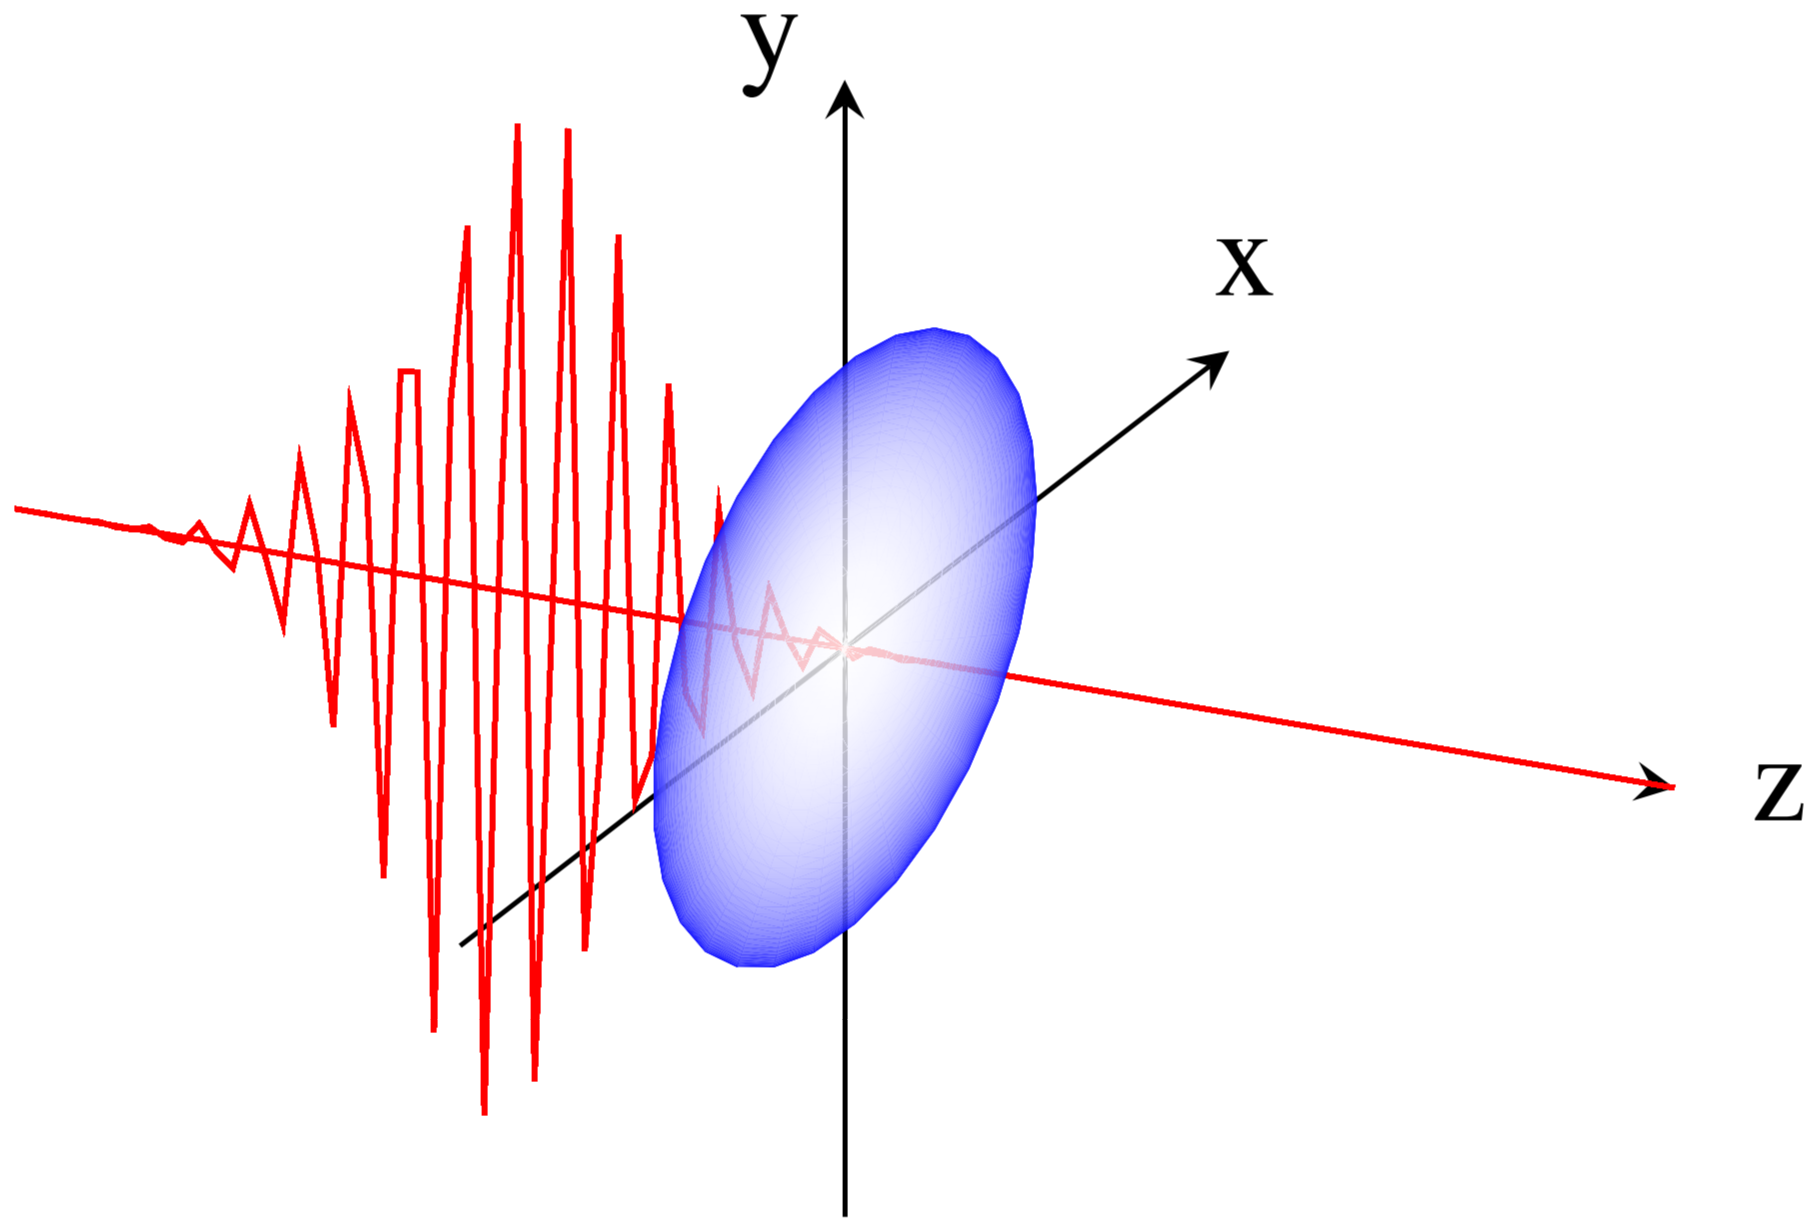
\includegraphics[width=0.40 \textwidth]{figs/Fig_1a.png}
\hspace{1cm}
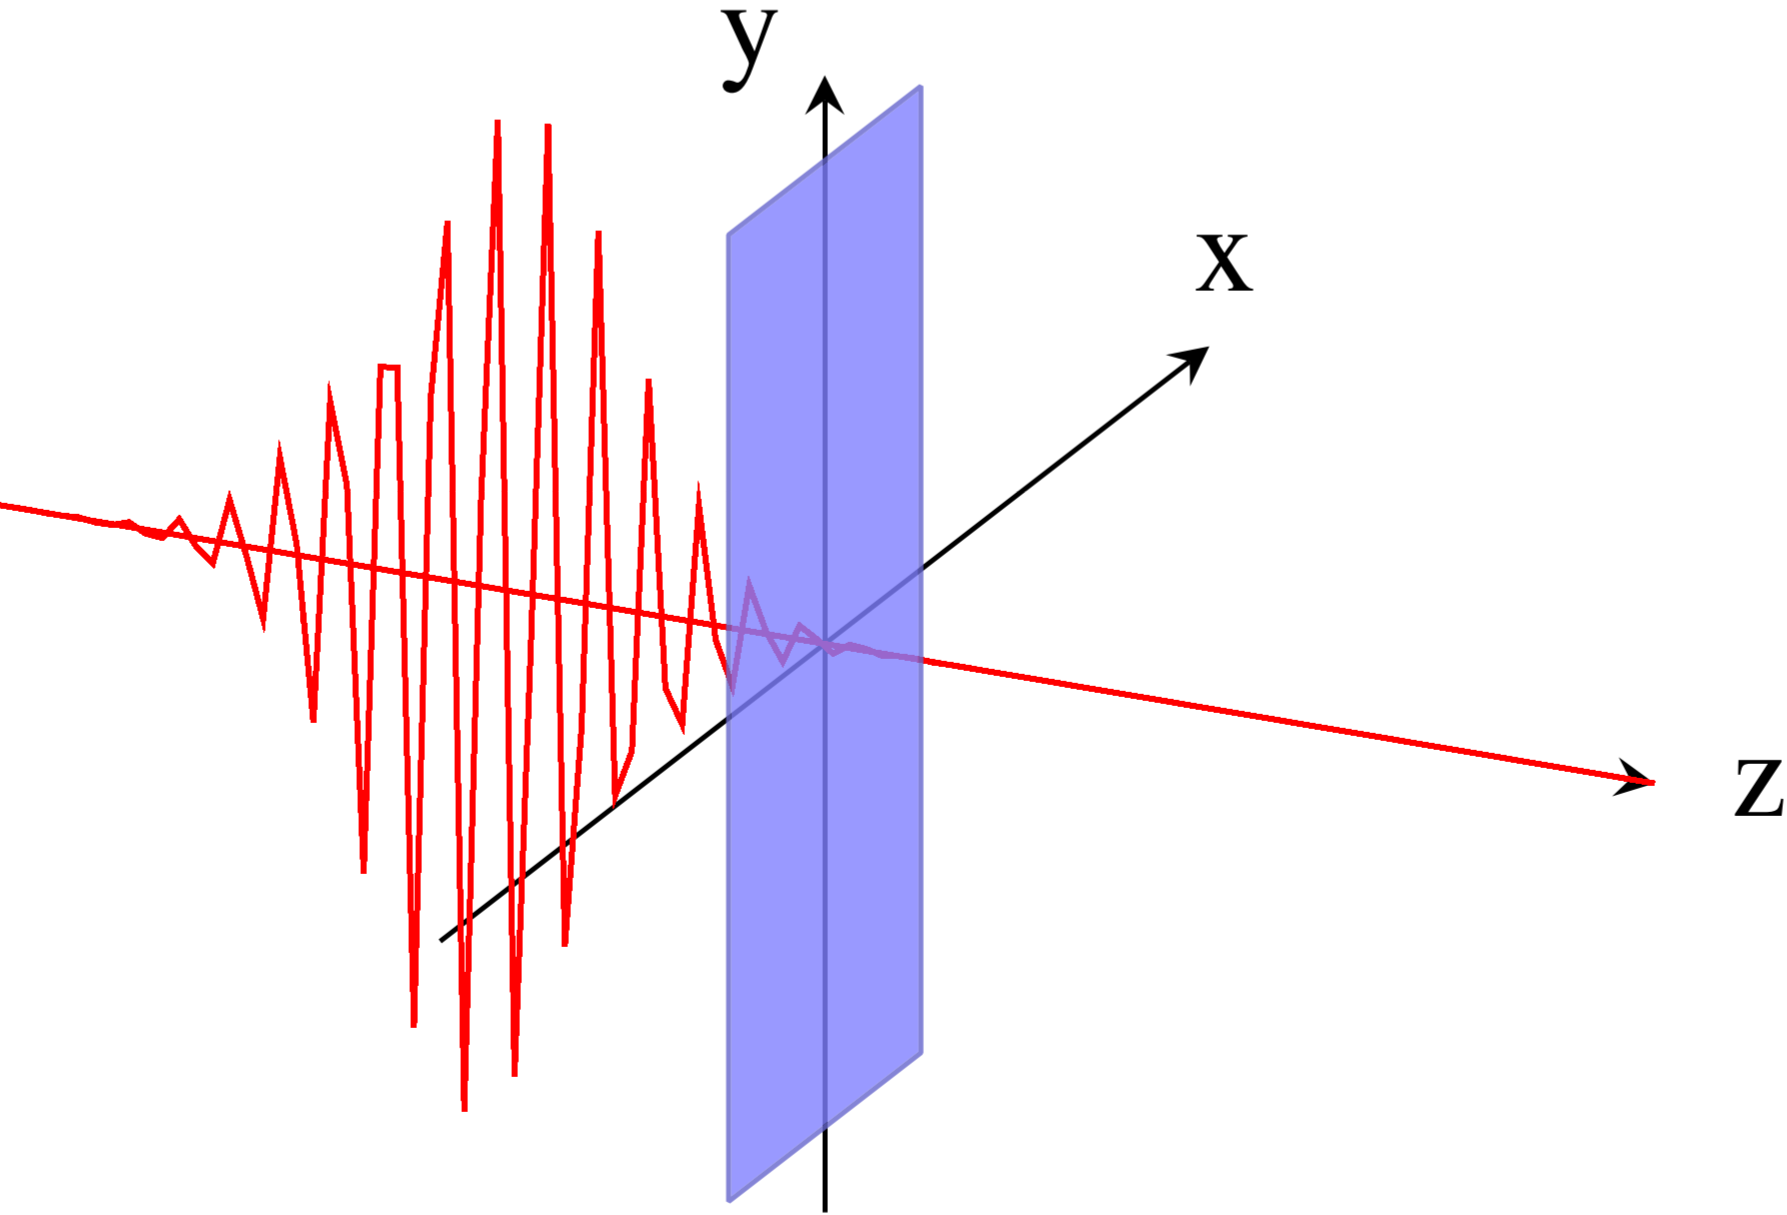
\includegraphics[width=0.40 \textwidth]{figs/Fig_1b.png} 
\caption{
  Left: 3D case (charge on a disc of radius $R$). Right: 2D case (charge on a strip of infinite length).
}
\end{figure} 
\end{frame}





%\subsection{The 3D case}
\begin{frame}{Proposed laws}{The 3D case}

Laser pulse: propagates along the $z$ axis

Hypothesis: electrostatic potential $V$ which vanishes at $z=0$, where a uniform charge density $\sigma$, within a disc of radius $R$, is located.
%
\[ V(\zeta)= 2\pi R\,\sigma\,\Bigl( \sqrt{1+\zeta^2} -\zeta -1 \Bigr ) \qquad \qquad
\zeta={z\over R} \]
%

\vspace{5mm}
A particle initially at rest accelerates and the law of motion is obtained from energy conservation. Since $V(0)=0$, we have 
%
\[ m{v^2\over 2} +eV(z)=0 \qquad \quad v=\dot z \]
\end{frame}





\begin{frame}{Proposed laws}{The 3D case}
so that

\[ 
   E_\infty= m{v_\infty^2\over 2}=2\pi eR\sigma \hspace{1cm} v_\infty=\dot{z}(\infty) 
\]

The kinetic energy of the particle, after integrating the equation of motion, is
%
\[ E_{\mathrm{kin}}(t) \simeq E_\infty\parton{ 1-{t^*\over t}}^2 \qquad \quad t>t^*
= {R\over 4v_\infty}\]
%

Since this is an asymptotic law, we may assume that $E(t)=0$ for $t<t^*$.
\end{frame}





%\subsection{The law to be fitted for 3D simulations}
\begin{frame}{Proposed laws}{Fits for 3D simulations}
\[
\left\{
  \begin{array}{ll}
    \displaystyle \Emax^{(3D)}(ct) = 0                                                   &\mathrm{for}\; t<t^{*(3D)} \\
    \displaystyle \Emax^{(3D)}(ct) = E^{(3D)}_\infty\,\parton{ 1-{ct^{*(3D)}\over ct}}^2 &\mathrm{for}\; t>t^{*(3D)}
  \end{array}
\right.
\]
%
We can perform a linear fit by defining $y=\sqrt{E}$ and $x=1/ct$, so that the previous law
becomes
%
\[ y=a+bx \qquad \qquad \qquad E^{(3D)}_\infty=a^2 \qquad ct^{*(3D)}= -{b\over a} \]
%
\end{frame}



%\subsection{The 2D case}
\begin{frame}{Proposed laws}{The 2D case}
Laser pulse: propagates along the $z$ axis

Hypothesis: electrostatic potential $V$ which vanishes at $z=0$, where a uniform charge density $\sigma$, on an infinite strip along the $y$ axis and with a size $R$ along the $x$ axis, is located.

\[
  \begin{split}
    \displaystyle V(z) &= 4R\sigma \parton{-\zeta \arctan {1\over \zeta} +\log{1\over\sqrt{1+\zeta^2}} }\\
    \displaystyle &\simeq -4R\sigma\, \log(1+\zeta)
  \end{split}
\]
where we defined \(\zeta=z/R\).
\end{frame}




\begin{frame}{Proposed laws}{The 2D case}
%To obtain this result, it is simpler to compute first the electric field $\Ecal_x= 4\sigma\,\, \arctan(1/\zeta)$, whose asymptotic behaviour is $4\sigma/\zeta$. As a consequence, a potential having this asymptotic  behaviour and which vanishes at the origin is  $\hat{V}\simeq -4R\sigma\, \log(1+\zeta)$. 
The potential in this case diverges logarithmically and consequently the particle accelerates indefinitely. We approximate the potential energy with
%
\[ e\hat{V}(z)= - E_\infty\, \log(1+\zeta) \]

so that

\[
E_\infty\equiv m{v_\infty^2\over 2}= 4eR\sigma 
\]

Integrating the equations of motion we have
\[
  E_{\mathrm{kin}}(t)= E_\infty \log\parton{t\over t^*} \qquad \qquad t\geq t^*= {R\over v_\infty} 
\]

Since this is an asymptotic law, we may assume that $E(t)=0$ for $t<t^*$. 
\end{frame}





%\subsection{Law to be fitted for 2D simulations}
\begin{frame}{Proposed laws}{Fits for 2D simulations}
%
\[
\left\{
  \begin{array}{ll}
    \displaystyle \Emax^{(2D)}(ct) = 0                                   &\mathrm{for}\; t<t^{*(2D)} \\
    \displaystyle \Emax^{(2D)}(ct) = E^{(2D)}_\infty\,\log{ct\over ct^*} &\mathrm{for}\; t>t^{*(2D)}
  \end{array}
\right.
\]
%
We perform a linear fit by defining $y=E$ and $x=\log ct$, so that the previous law
becomes
%
\[ y=a+bx \qquad \qquad \qquad E^{(2D)}_\infty=b \qquad ct^{*(2D)}=e^{-a/b} \]
%
\end{frame}




%\section{Results for 2D simulations}
\begin{frame}{Results for 2D simulations}{Normal incidence, different target thicknesses}
\begin{figure}
\centering
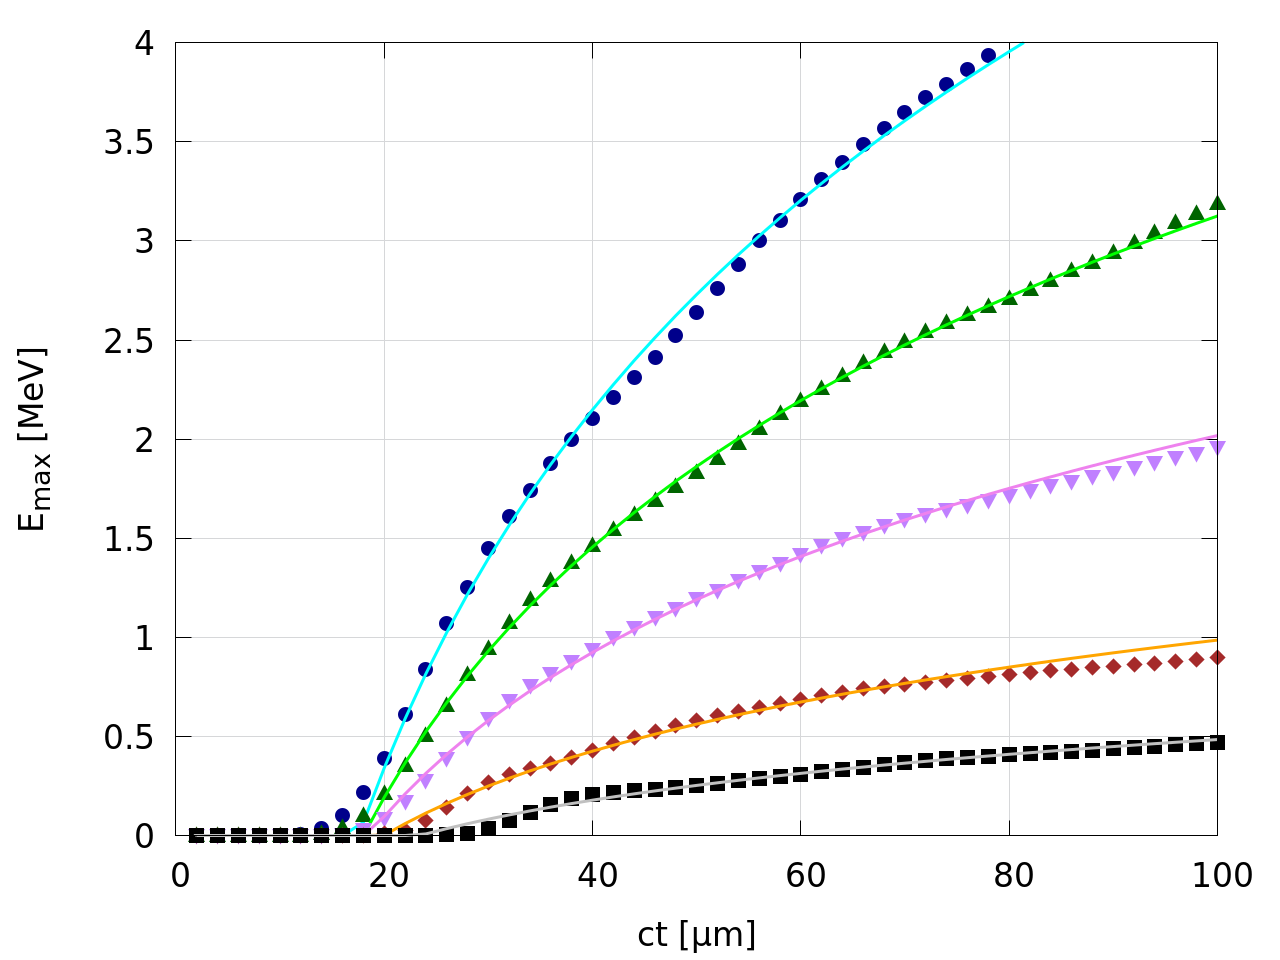
\includegraphics[width=0.45 \textwidth]{figs/Fig_2a.png}
\hspace{5mm}
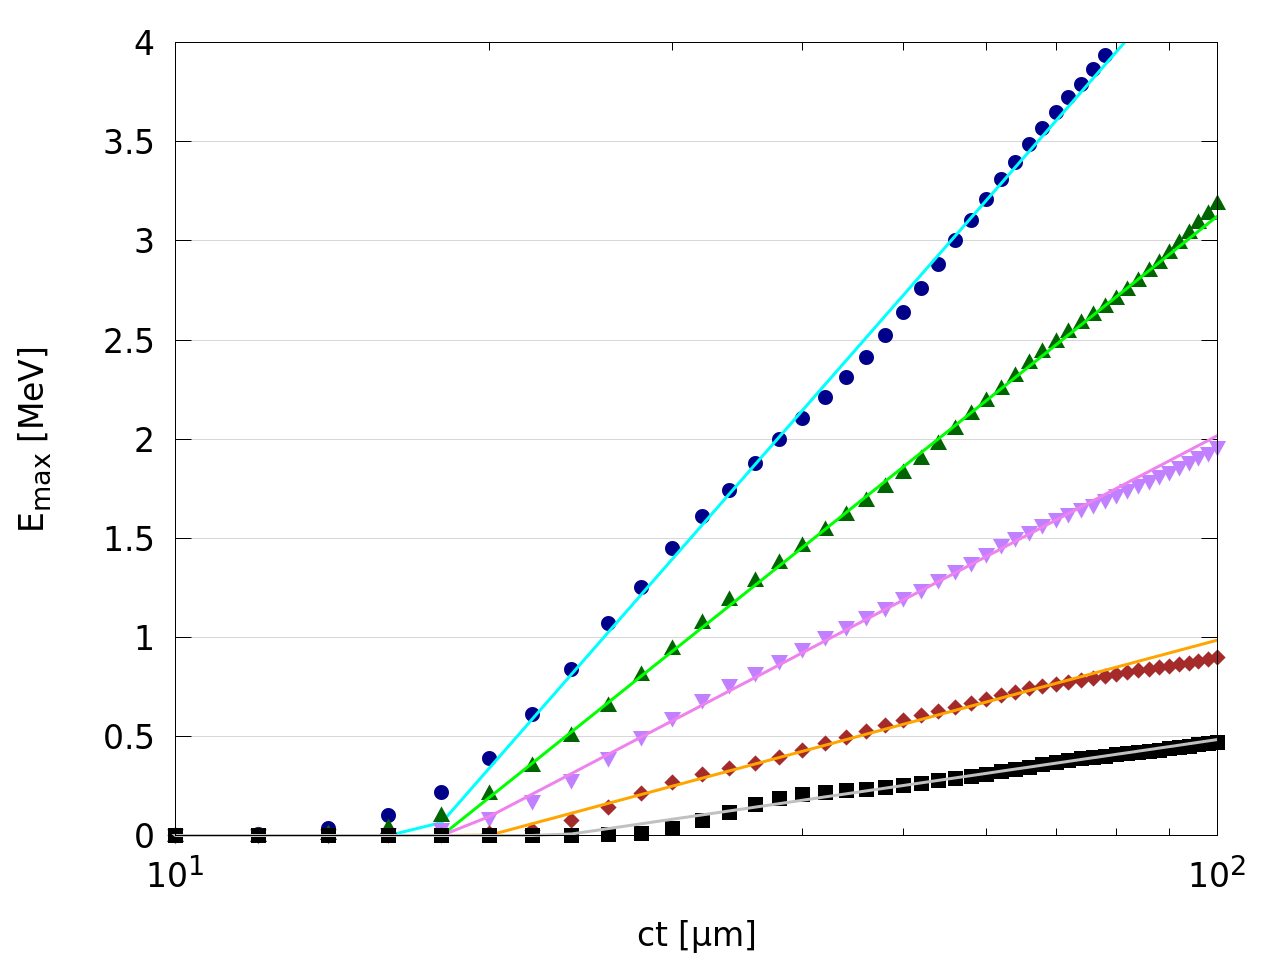
\includegraphics[width=0.45 \textwidth]{figs/Fig_2b.png} 
\caption{
Left: $\Emax$ versus $ct$, PIC simulation (symbols) vs fit (continuous line): blue $L=0.5 \,\mu$m, green $L=1 \,\mu$m, violet $L=2 \,\mu$m, orange $L=4 \,\mu$m, black $L= \,8\mu$m. Right: the same as the left panel but in a logarithmic scale for $ct$ which clearly shows the linearity and the accuracy of the fit.
}
\end{figure} 
\end{frame}




%\section{Results for 2D simulations - extended}
\begin{frame}{Results for 2D simulations}{Non-normal incidence, fixed target thickness}
\begin{figure}
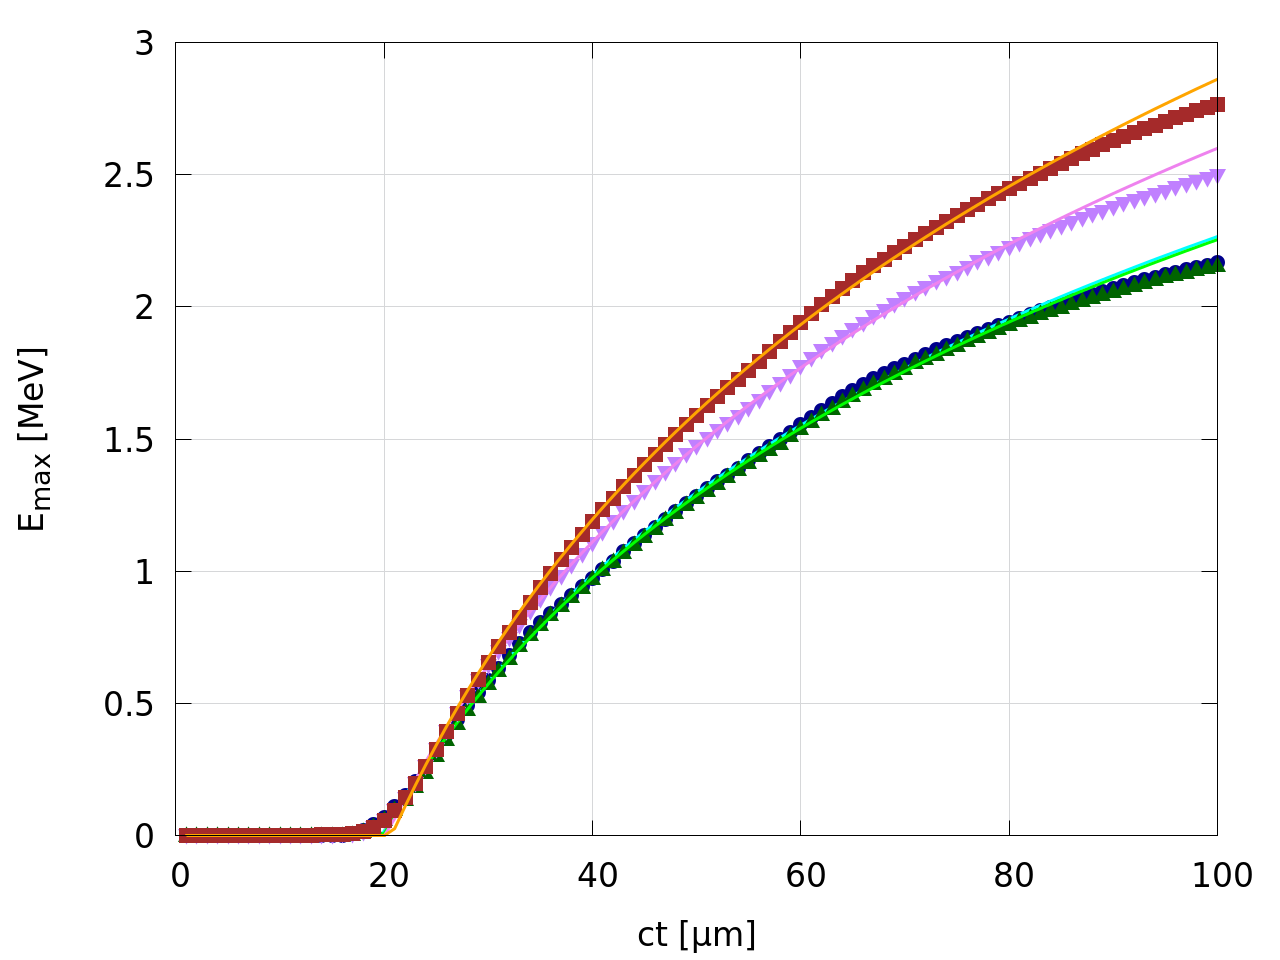
\includegraphics[width=0.45 \textwidth]{figs/Fig_4a.png}
\hspace{5mm}
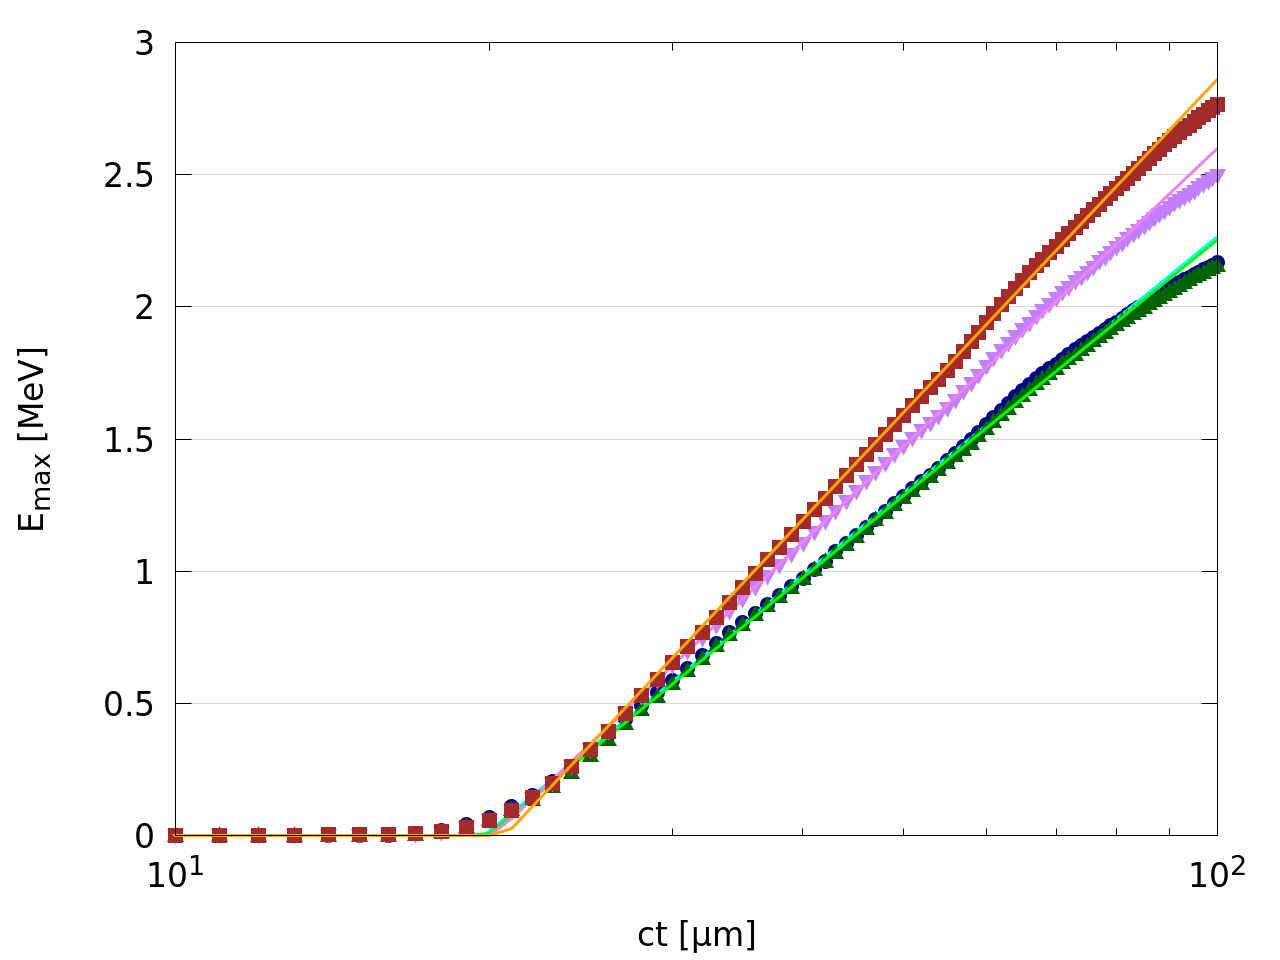
\includegraphics[width=0.45 \textwidth]{figs/Fig_4b.png}
\caption{
Left: $\Emax$ versus $ct$, PIC simulation (symbols) vs fit (continuous line): $\alpha=5^{\circ}$ green, $\alpha=10^{\circ}$ violet and $\alpha=15^{\circ}$ orange. Right: the same data are plotted as with a logarithmic scale for $ct$, which shows how the data stay on a line and the accuracy of the linear fit.
}
\end{figure}
\end{frame}





%\section{Results for 3D simulations}
\begin{frame}{Results for 3D simulations}{Normal incidence, different target thicknesses}
\begin{figure}
\centering
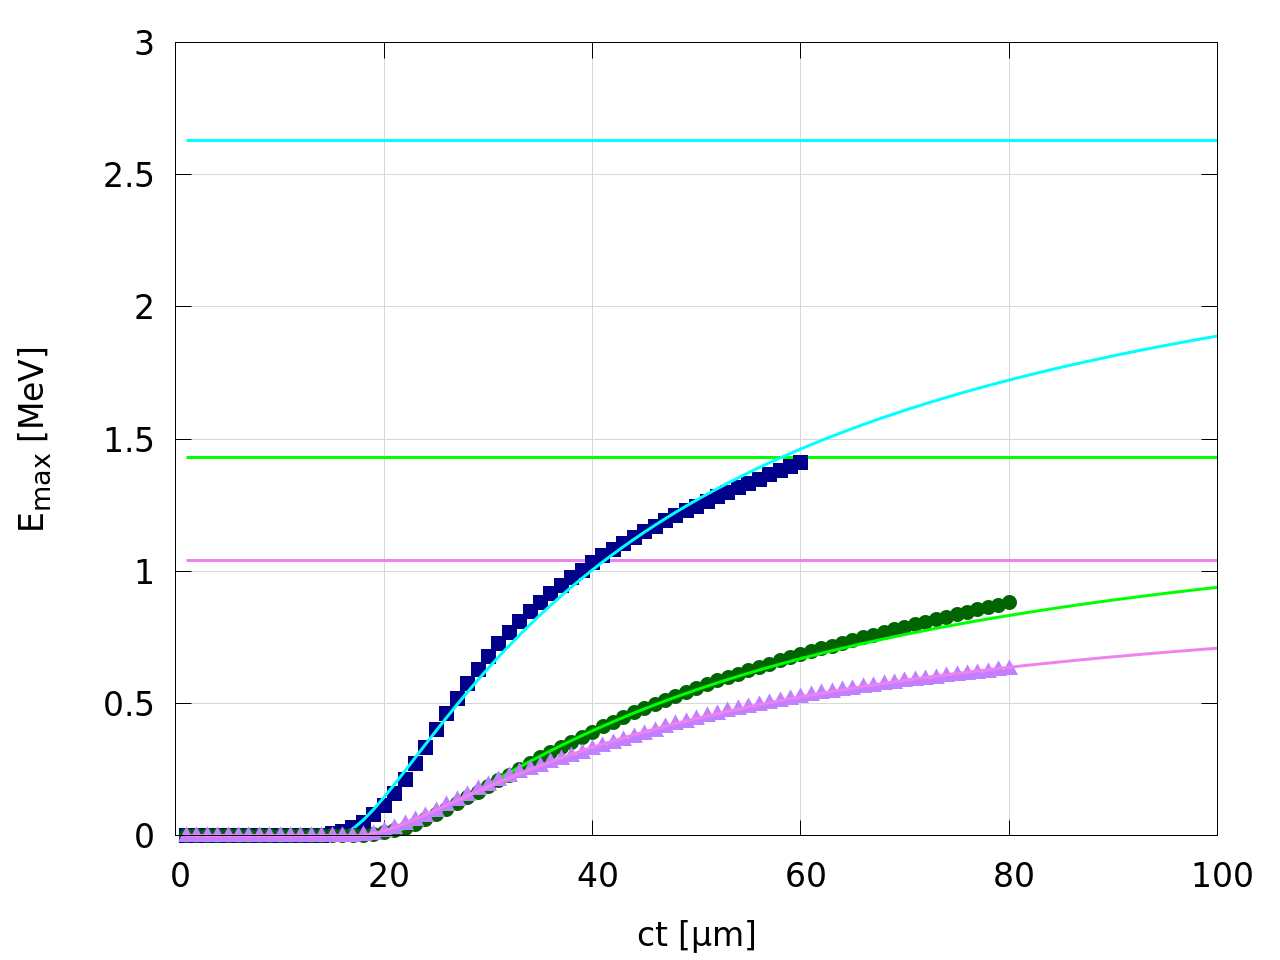
\includegraphics[width=0.45 \textwidth]{figs/Fig_5b.png}
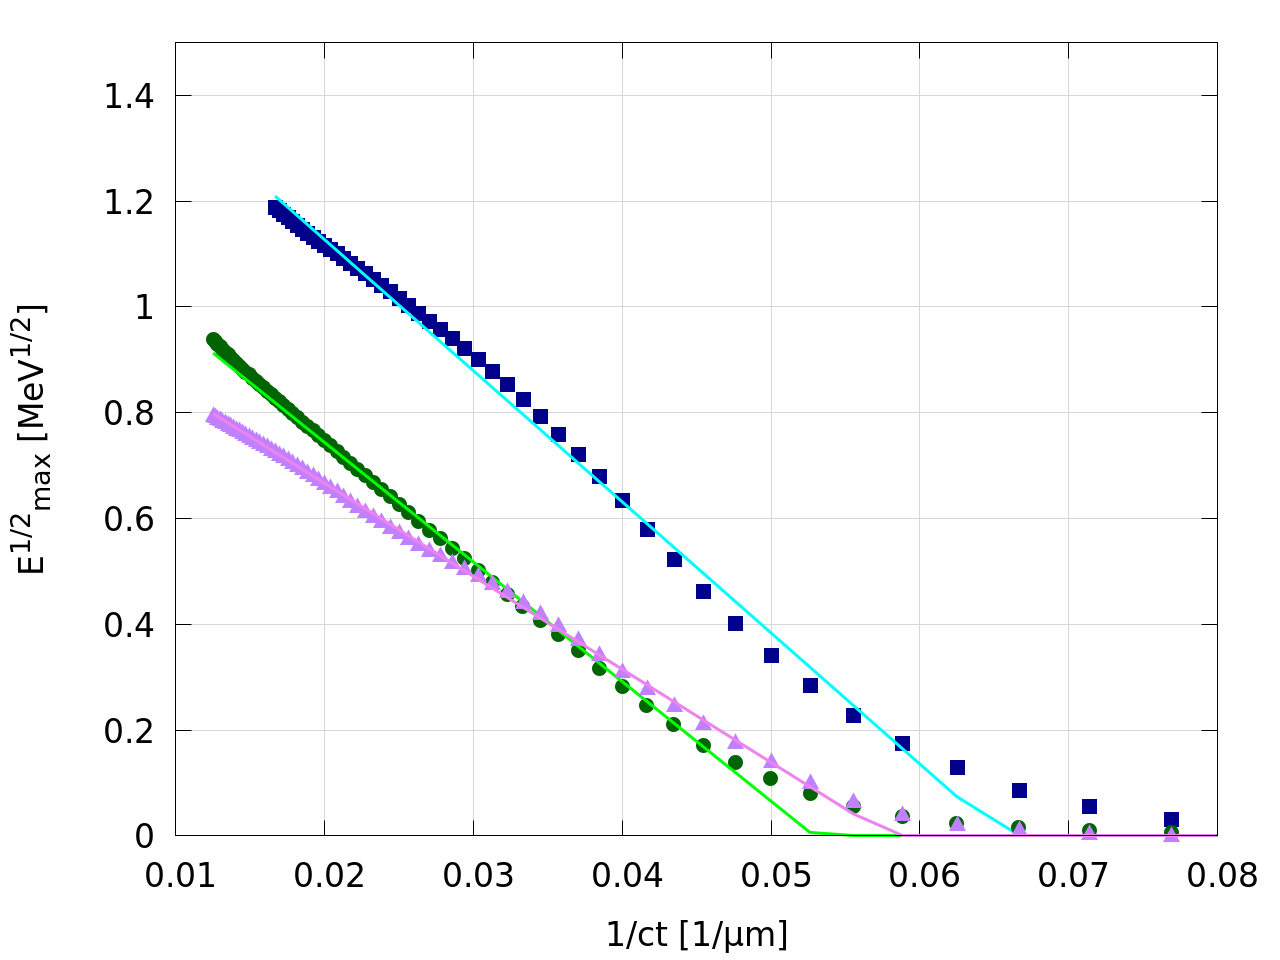
\includegraphics[width=0.45 \textwidth]{figs/Fig_6.png}
\caption{
Left: $\Emax$ versus $ct$, PIC simulation (symbols) vs fit (continuous line): $L=0.5 \mu$m blue, $L=1 \mu$m green and to $L=2 \mu$m violet. Right: Plot of $\sqrt{E_{\mathrm{max}}}$ versus $1/ct$ which shows their linearity and the accuracy of the fit.
}
\end{figure}
\end{frame}




%\section{Comparison with experiments}
\begin{frame}{Comparison with experiments}{Where are we?}
\begin{figure}
\centering
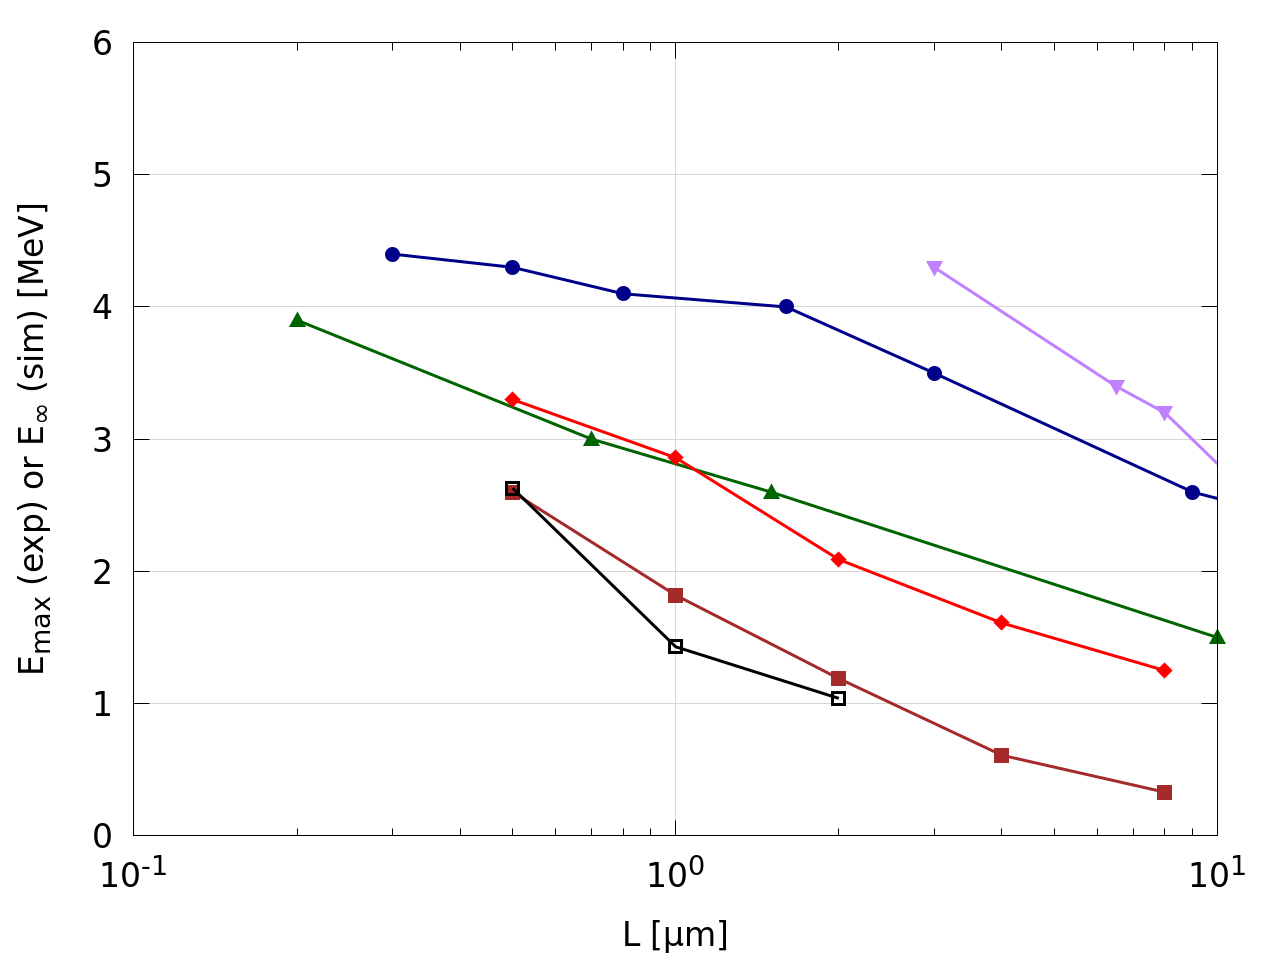
\includegraphics[width=0.45 \textwidth]{figs/Fig_7.png}
\caption{
$\Emax$ versus $L$ from various experiments ($a_0 \sim 3$ and a metal target): Ceccotti's (45$^\circ$ incidence angle) (blue), Neely's  (30$^\circ$) (green), Flacco's (45$^\circ$) (violet), fits from our 2D PIC simulation at zero degree incidence (brown), fits from 2D sims at 30$^\circ$ incidence (red) and fits from 3D PIC simulation at zero degree incidence (black).
}
\end{figure}
\end{frame}


%\section{Results}
\begin{frame}{Conclusions}{What we knew}

\begin{itemize}
\item The asymptotic value of the cut-off energy of protons, which is what is measured in experiments, is difficult to extract from PIC simulations
\item The 2D results do not exhibit a saturation
\item The 3D results show that a saturation might be reached, despite at a large time ($ct > 200\,\mu$m), which is computationally too expensive
\end{itemize}

\end{frame}



\begin{frame}{Conclusions}{What is new}

\begin{itemize}
\item We formulated two empirical laws for 2D and 3D simulations, which depend on the asymptotic energy $E_\infty$
\item The fits to the 2D and 3D results coming from PIC simulations are quite good and the statistical uncertainties are a few percent
\item The extrapolated values $E_{\infty}^{2D}$ and $E_{\infty}^{3D}$ are comparable
\item $E_{\infty}^{2D}$ and $E_{\infty}^{3D}$ can be fully calculated fitting the results obtained before $ct \leq 50 \sim 60\,\mu$m, which is a distance reachable also in 3D simulations
\end{itemize}

\end{frame}



\begin{frame}{Conclusions}{What is new}

\begin{itemize}
\item The fitting appears to be satisfactory also for small incidence angles, even though the model was developed for normal incidence
\item The proposed phenomenological model is adequate to avoid the arbitrariness in the choice of the time at which the asymptotic cut-off energy is chosen in numerical simulations
\item 2D simulations may have a quantitative value, with an adequate extrapolation, rather than being of purely qualitative nature
\end{itemize}

\end{frame}



\end{document}



\appendix
\backupbegin




{ % all template changes are local to this group.
    \setbeamertemplate{navigation symbols}{}
    \begin{frame}[plain]
        \begin{tikzpicture}[remember picture,overlay]
            \node[at=(current page.center)] {
                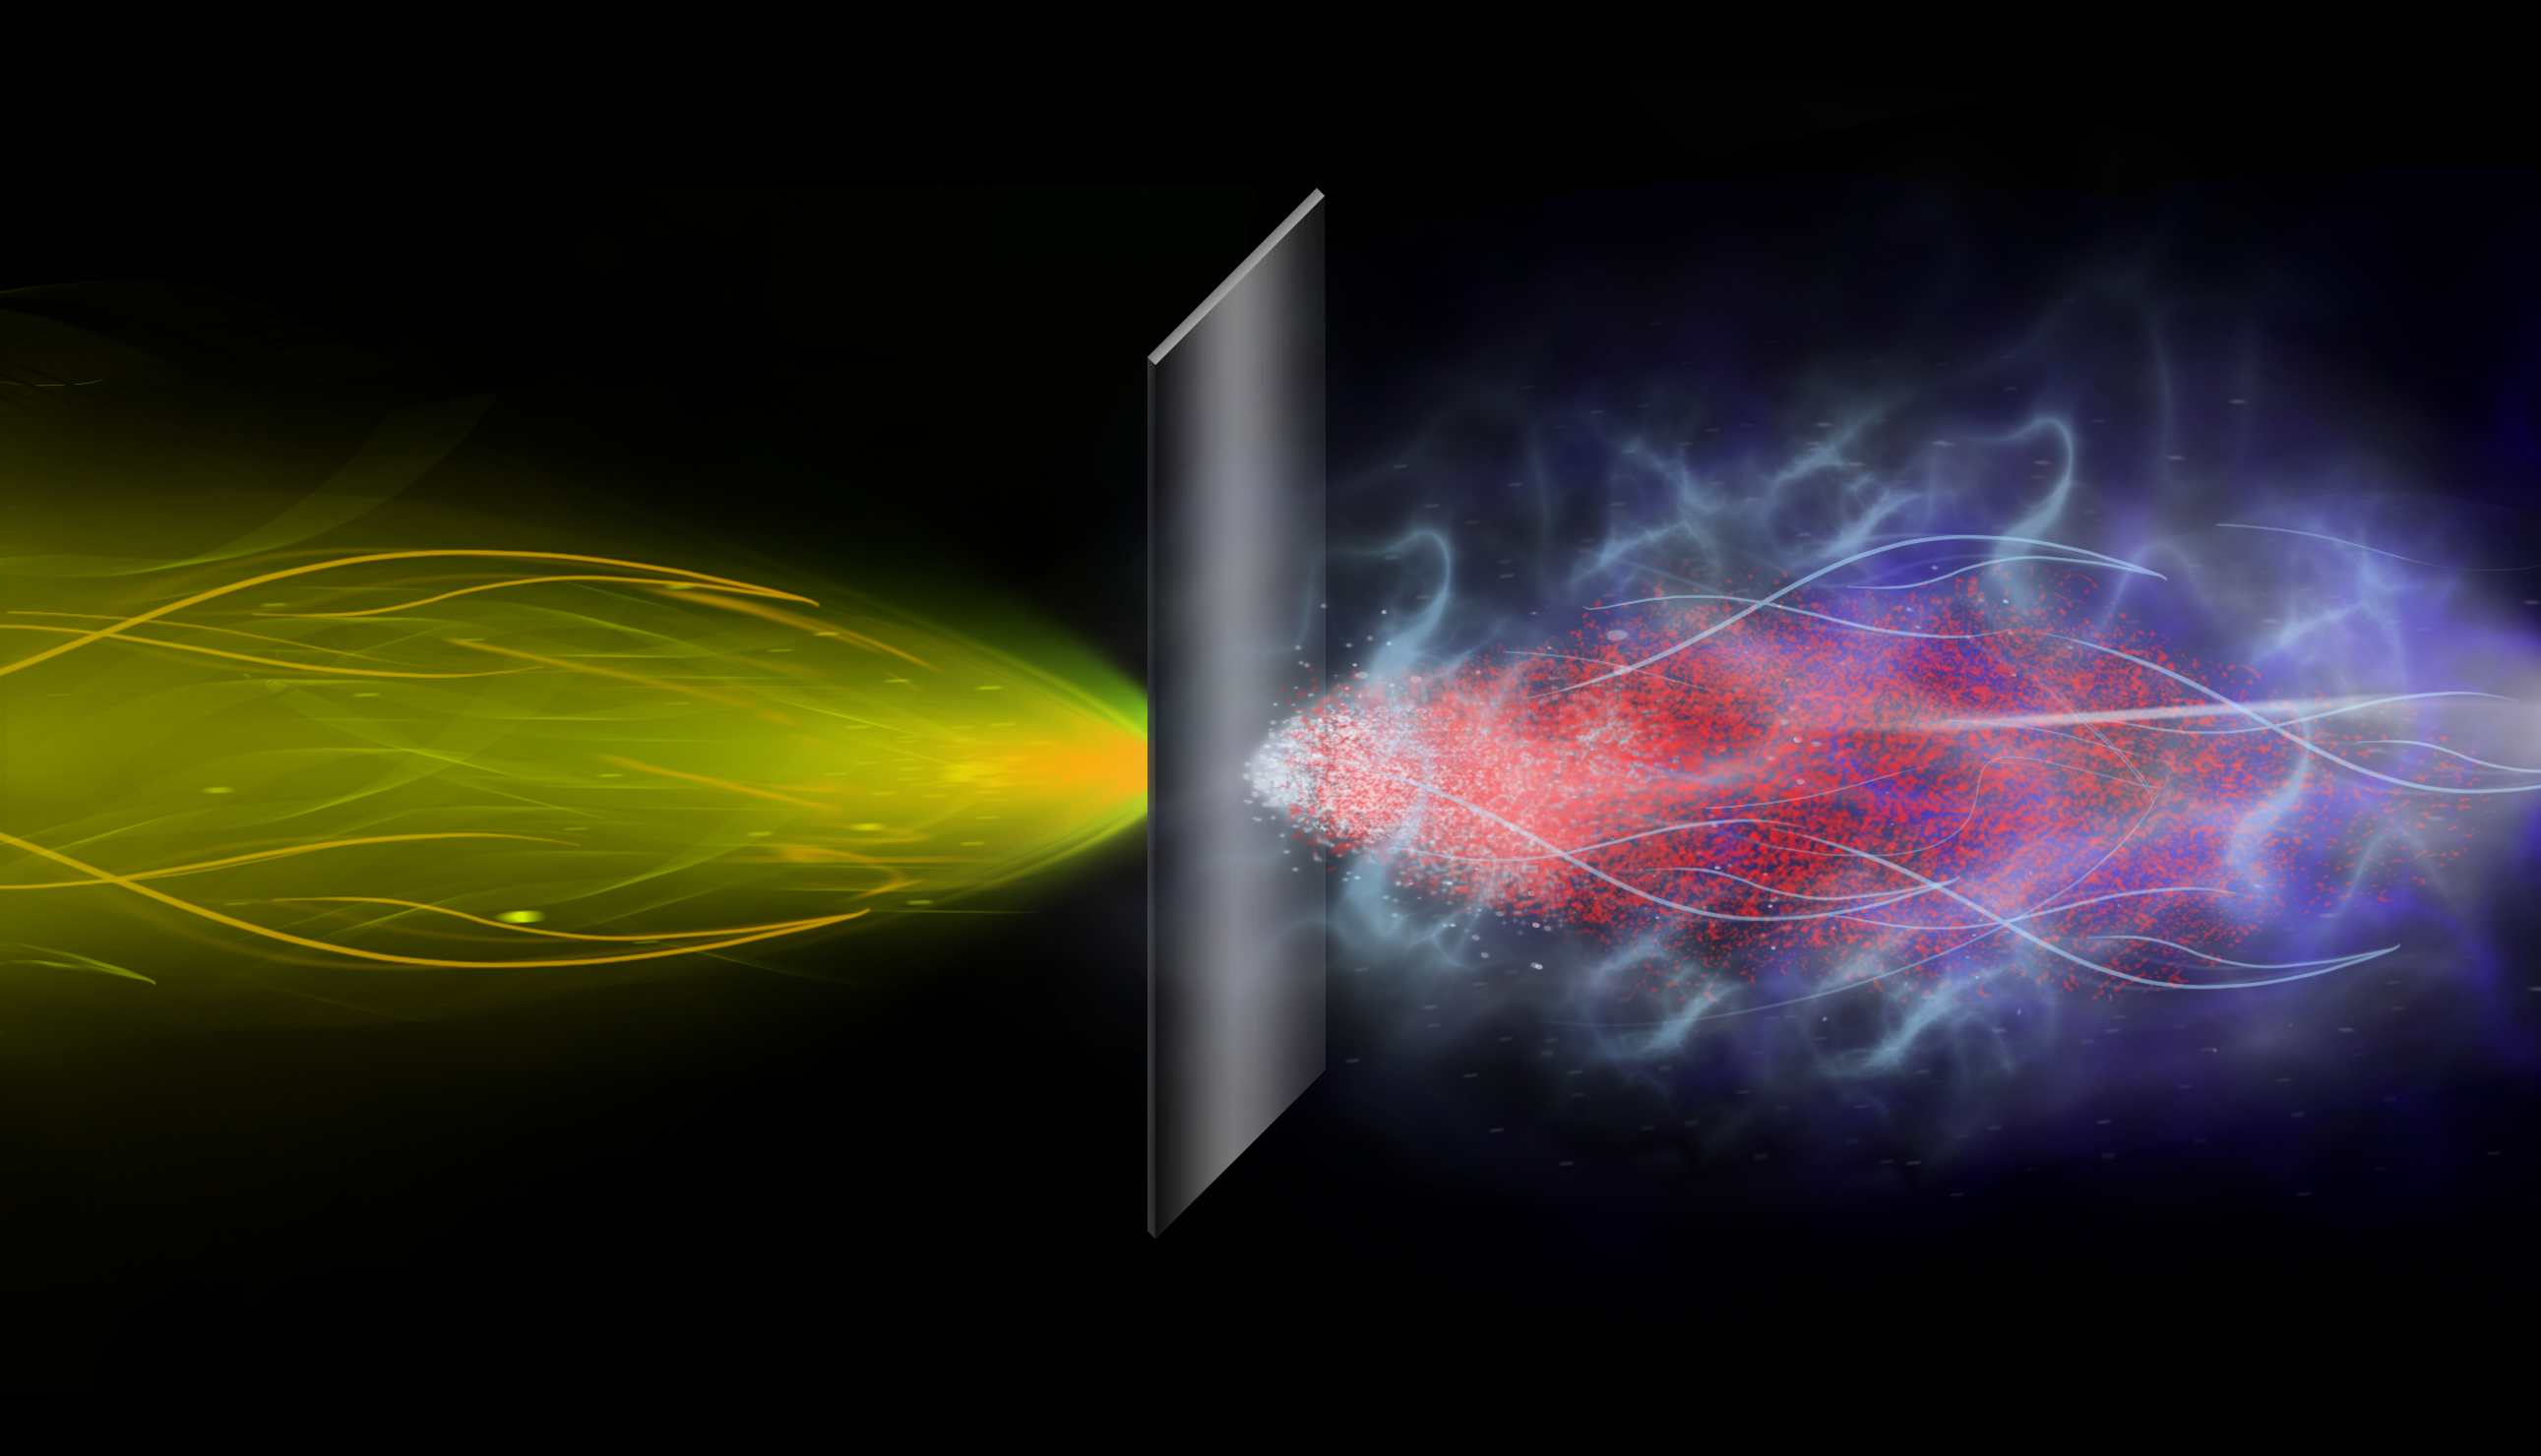
\includegraphics[width=\paperwidth]{figs/tnsa.png}
            };
        \end{tikzpicture}
        \vspace{10cm}
        \scriptsize{Freely inspired by A. Macchi et al. (2013)}
     \end{frame}
}




\begin{frame}
\end{frame}




\begin{frame}{Results for 2D simulations}
\begin{figure}
\centering
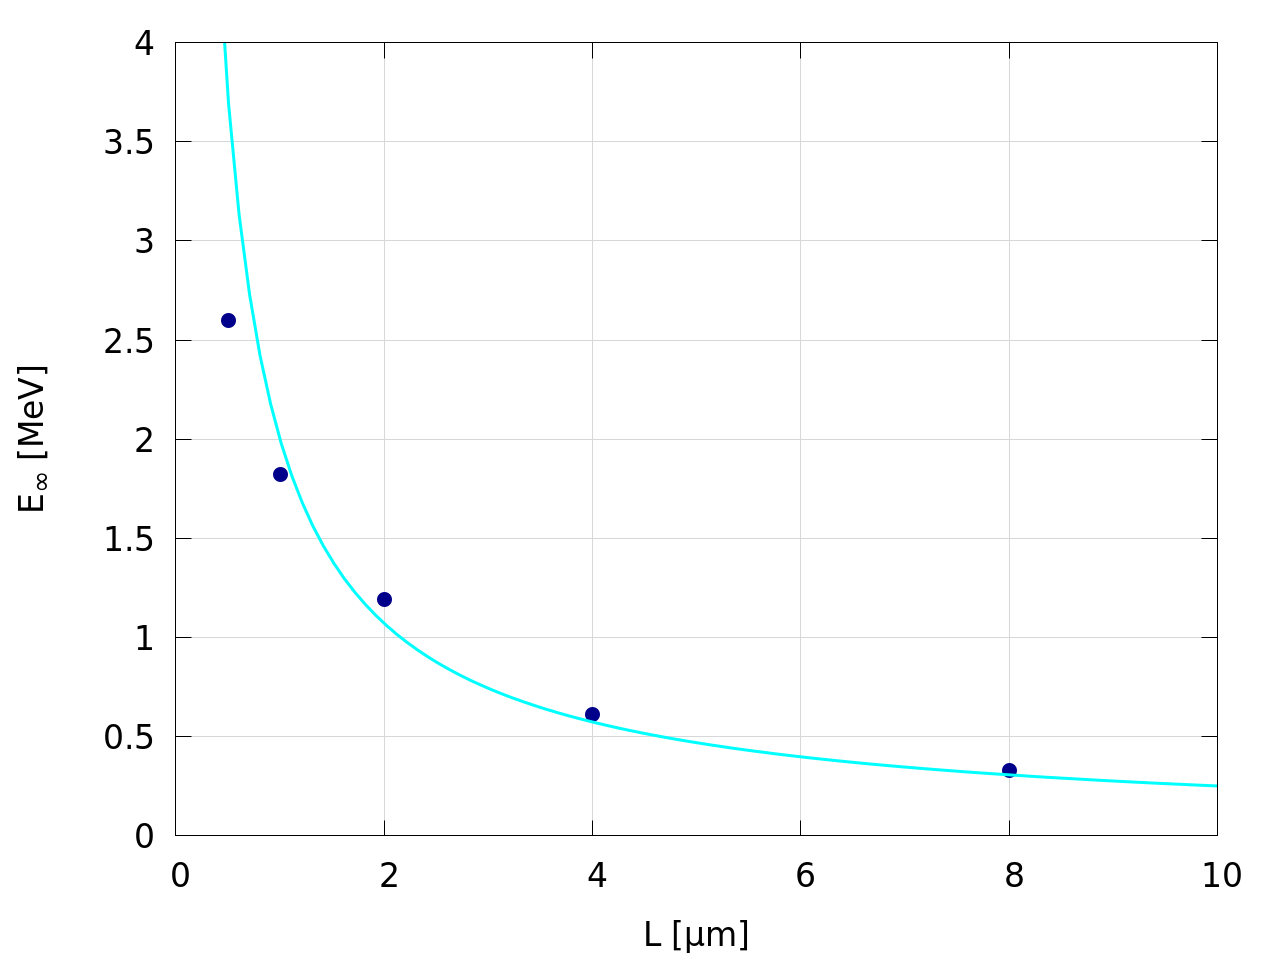
\includegraphics[width=0.45 \textwidth]{figs/Fig_3.png}
\caption{
Comparison of the extrapolated cut-off energy for 2D PIC simulations (symbols) for different target thicknesses $L=0.5, 1,2,4,8 \mu$m
and a fit with the curve $E_{\mathrm{max}}=1/L^{0.9}$ (cyan line).
}
\label{fig:3} 
\end{figure}
\end{frame}




\begin{frame}{Comparison with experiments}{Fits for 2D simulations with normal incidence angle and different thicknesses}
\begin{table}[ht]
\centering 
\begin{tabular}{c c c c c c }
\hline \hline 
$L$ & $\Emax(ct=50)$ & $E_\infty^{(2D)}$ & $ct^{*(2D)}$ & $\sigma_E$ & $\sigma_{ct^*} $ \\ [0.5ex] % inserts table heading
\hline 
 0.5 & 2.64 & 2.62 & 17.5 & 0.05 & 0.03 \\
 1 & 1.82 & 1.82 & 18.0 & 0.02 & 0.15 \\
 2 & 1.19 & 1.19 & 18.4 & 0.02 & 0.2 \\
 4 & 0.58 & 0.61 & 19.9 & 0.02 & 0.5 \\
 8 & 0.25 & 0.33 & 23.3 & 0.02 & 0.9 \\
\hline 
\end{tabular}
\end{table}
\end{frame}




\begin{frame}{Comparison with experiments}{Fits for 2D simulations with non-normal incidence angles and fixed thickness}
\begin{table}[ht]
\centering 
\begin{tabular}{c c c c c c }
\hline \hline 
$\alpha$ & $\Emax(ct=50)$ & $E_\infty^{(2D)}$ & $ct^{*(2D)}$ & $\sigma_E$ & $\sigma_{ct^*} $ \\ [0.5ex] % inserts table heading
\hline 
 5 & 1.28 & 1.40 & 19.9 & 0.01 & 0.1 \\
 10 & 1.47 & 1.62 & 20.1 & 0.01 & 0.1 \\
 15 & 1.59 & 1.82 & 20.7 & 0.02 & 0.15 \\
\hline 
\end{tabular}
\end{table}
\end{frame}



\begin{frame}{Comparison with experiments}{Fits for 3D simulations with normal incidence angle and different thicknesses}
\begin{table}[ht]
\centering 
\begin{tabular}{c c c c c c }
\hline \hline 
$ L $ & $\Emax(ct=50)$ & $E_\infty^{(3D)}$ & $ct^{*(3D)}$ & $\sigma_E$ & $\sigma_{ct^*} $ \\ [0.5ex] % inserts table heading
\hline 
 0.5 & 1.25 & 2.63 & 15.3 & 0.01 & 0.2 \\
 1 & 0.56 & 1.43 & 18.9 & 0.02 & 0.1 \\
 2 & 0.44 & 1.04 & 17.3 & 0.01 & 0.1 \\
\hline 
\end{tabular}
\end{table}
\end{frame}




%\section{Behind the scenes}
%\subsection{Initial densities}
\begin{frame}{Behind the scenes}{The 3D case: Initial densities}
Let's consider a target which is infinitely extended along the plane $xy$ and delimited by the planes $z=-L$ and $z=0$.  We can consider a circular radius $r_L$ which we assume to be the spot of the laser  pulse propagating along $z$. The electrons are heated and diffused by the laser itself. Supposing  that they diverge with angle $\theta$, the electrons will leave the plane $z=0$ from a disc of radius 
%
\[ R= r_L + L \tan \theta \]
%
\end{frame}



\begin{frame}{Behind the scenes}{The 3D case: Initial densities}
We assume that the target is a metallic foil and that the protons are in the contaminants deposited on the plane $z=0$.
The electrons are heated, diffuse and cross the $z=0$ boundary leaving the target and inducing on it a positive charge density $\sigma(t)$, that we suppose varies slowly with $t$. If $Qe$ is the total number of positive charge on the surface, the density is
%
\begin{equation}
\sigma= { Q e\over \pi \,R^2}
\label{eq:3d_density}
\end{equation}
%
This is the geometry for the 3D case, that we shall treat analytically
\end{frame}




\begin{frame}{Behind the scenes}{The 2D case: Initial densities}
We consider another geometry in which the electrons on the plane $z=L$ leave the rectangle $|x|\leq R$, $|y|\leq L$ of area $4LR$. In this case the density is given by 
%
\begin{equation}
\sigma= { Q e\over 4 RL}
\label{eq:2d_density}
\end{equation}
%
The intensity defined as the power per unit surface is assumed to be the same for both geometries.
\end{frame}



%\section{The 3D case: charge density on a disk}
\begin{frame}{Behind the scenes}{The 3D case: charge density on a disk}
Using cylindrical coordinates and computing the potential we have
%
\[
\begin{split}
V(z) &= 2\pi\sigma \,\int_0^R \,r dr {1\over \sqrt{r^2+z^2}}= \pi \sigma \int_0^R \,dr^2 {1\over \sqrt{ z^2+r^2}}= \\
&= 2\pi \sigma \left[ \sqrt{z^2+R^2} -z \right]
\end{split}
\]
%
Introducing the dimensionless variable $\zeta= z/R$ we have
%
\[
V(\zeta)= 2\pi\,R \sigma \left[ \sqrt{1+\zeta^2} -\zeta \right]
\]
\end{frame}




\begin{frame}{Behind the scenes}{The 3D case: charge density on a disk}
Since $V(0)= 2\pi\,R\,\sigma$ we redefine the potential by subtracting it.
%
\begin{equation}
\hat{V}(\zeta)= V(\zeta) - V(0) = 2\pi\,R \sigma \left[ \sqrt{1+\zeta^2} -\zeta -1 \right]
\label{eq:potential}
\end{equation}
%
\end{frame}




\begin{frame}{Behind the scenes}{The 3D case: charge density on a disk}
The potential energy is given by $eV(\zeta)$. We notice that we have 
\[
\left\{
  \begin{array}{ll}
    \displaystyle \hat{V}(z) \simeq -2\pi \sigma \,z              &\mathrm{for}\; z\to 0 \\
    \displaystyle \hat{V}(z) \simeq {eQ\over z} - {2Qe \over R}   &\mathrm{for}\; z\to \infty
  \end{array}
\right.
\]
%

Letting $v=\dot z$ and assuming $v(0)=0$, namely that the protons are initially at
rest on the surface $z=0$, we can apply the energy conservation
%
\[ m{v^2\over 2}+eV(\zeta)\equiv E+eV(\zeta)=0 \]
\end{frame}




\begin{frame}{Behind the scenes}{The 3D case: charge density on a disk}
Calling $v_\infty$ the speed reached at infinite distance
%
\[ E_\infty= m{v_\infty ^2\over 2} = -eV(\infty)= {2Qe^2\over R} = 2\pi \,e \, R\, \sigma \]
%
we can define
%
\[ -eV(\zeta)= 2\pi\,e\, R\sigma \,s(\zeta) = m{v_\infty ^2\over 2} s(\zeta) \]
%
where from equation \ref{eq:potential}
%
\[ s(\zeta)= 1+\zeta-\sqrt{1+\zeta^2} \]
%
As a consequence we have 
%
\begin{equation}
E= E_\infty s(\zeta) \qquad \qquad v=v_\infty \sqrt{s(\zeta)}
\end{equation}
\end{frame}




\begin{frame}{Behind the scenes}{The 3D case: charge density on a disk}
We introduce the new variables
%
\[ X=\sqrt{s} \qquad \qquad \tau=t{ v_\infty \over R} \]
%
Then we have
%
\begin{equation} \label{eq:5}
{d\zeta\over d\tau}= {v\over v_\infty}= \sqrt{s(\zeta)}
\end{equation}
%
We might solve this equation with initial condition $\zeta(0)=0$. We rather solve the equation for $X$
%
\begin{equation} \label{eq:6}
{dX\over d\tau}= {dX\over ds}\,\,{ds\over d\zeta}\,\,{d\zeta\over d\tau}={1\over 2}\,{ds\over d\zeta}
\end{equation}
\end{frame}




\begin{frame}{Behind the scenes}{The 3D case: charge density on a disk}
Let us notice that
%
\[ {dX\over d\tau } = {1\over 2}\parton{1-{\zeta \over \sqrt{1+\zeta^2}}} = {1\over 2}\parton{ 1 +{\zeta\over 1-s}}^{-1} \]
%
inverting $s=s(\zeta)$ we have $\zeta= (2s-s^2)/(2(1-s))$ and finally replacing in the r.h.s. of the last equation we obtain 
%
\[ {dX\over d\tau } = \parton{ 1 +{1\over (1-s)^2}}^{-1} = \parton{ 1 +{1 \over (1-X^2)^2 }}^{-1} \]
%
\end{frame}



\begin{frame}{Behind the scenes}{The 3D case: charge density on a disk}
The results is obtained with integration by parts
\[
\begin{split}
\tau &= X + \int_0^ X {du\over (1 - u^2)^2} = \\
&= \left. X - {1\over 2}{d\over d\alpha} \,\int_0^X \,{1\over \alpha^2-u^2} \right |_{\alpha=1} = \\
&= X + {1\over 2}\,\, {X\over 1-X^2} + {1\over 4}\, \log{1+X\over 1-X}
\end{split}
\]
\end{frame}



\begin{frame}{Behind the scenes}{The 3D case: charge density on a disk}
Asymptotically, for $\tau\to \infty$, we have $X\to 1$
%
\[ \tau \sim {1\over 4(1-X) } \qquad \qquad X\simeq 1-{1\over 4\tau} \]
%
The energy asymptotic behaviour is given by $E/E_\infty= s=X^2$ and consequently for $t\to \infty$
%
\[ E\simeq E_\infty\,\parton{ 1-{1\over 4\tau}}^2 \]
\end{frame}




%\subsection{The 2D case: charge density on a strip}
\begin{frame}{Behind the scenes}{The 2D case: charge density on a strip}
We consider the slab $|x|\leq R$ and $|y|\leq L$ on the rear surface $z=0$ where the density is given by eq. (\ref{eq:2d_density}). The potential is given by
%
\begin{equation} \label{eq:2d_potential}
\begin{split}
V(z) &= \sigma \int_{-R}^R \,dx \int_{-L}^L\,{dy \over \sqrt{x^2+y^2+z^2}} = \\
&= 4 \sigma \int_0^R \,dx \int_0^{L/\sqrt{x^2+z^2}}\,{du\over \sqrt{1+u^2}} = \\
&= 4\sigma \, \int_0^R \,dx\,\mathrm{arsinh}\parton{L\over \sqrt{x^2+z^2}}
\end{split}
\end{equation}
\end{frame}





\begin{frame}{Behind the scenes}{The 2D case: charge density on a strip}
Since $4\sigma= eQ/(LR)$, we first consider the limit $L\to 0$, which corresponds to the density $\sigma(z)= {eQ/(2R)}\delta(y)$, and the result, letting $\zeta=z/R$, is
%
\[ V(z)= {eQ\over R}\,\, \int_0^R \,dx\,\parton{1\over \sqrt{x^2+z^2}} = {eQ\over R}\,\mathrm{arsinh}{1\over \zeta}\]
\end{frame}




\begin{frame}{Behind the scenes}{The 2D case: charge density on a strip}
Since
\[ 
   \mathrm{arsinh}(u)= \log(u+\sqrt{1+u^2})
\]
we see that 
\[
  V(\zeta)\sim \log(2/\zeta) \text{ for } \zeta \to 0
\]
whereas it vanishes as $1/\zeta$ for $\zeta \to \infty$. As a consequence we cannot have $V$ vanishing at $\zeta=0$ with a subtraction. Indeed, if we compute $V(0)$, we will see that it diverges as $\log (1/L)$ for $L\to 0$ (see eq. \ref{eq:diverging_potential_as_log}).
\end{frame}


\begin{frame}{Behind the scenes}{The 2D case: charge density on a strip}
We wish to define a potential which vanishes at $z=0$: as a consequence, in the definition, we have to subtract $V(0)$. This can be done for any finite value of $L$ and also for $L\to \infty$. In order to compute $V(0)$ for a given non vanishing $L$, we set $\xi=x/L$; integrating by parts we obtain
%
\begin{equation} \label{eq:10}
\begin{split}
V(0) &= {eQ\over R}\,\int_0^{R/L} \,d\xi \,\mathrm{arsinh}{1\over \xi} \\
&= {eQ\over R} \parqua{ \left. \xi\mathrm{arsinh}{1\over \xi}\right |_0^{R/L} +\int_0^{R/L} {d\xi\over \sqrt{1+\xi^2}} } = \\
&= {eQ\over R} \parqua{ {R\over L} \mathrm{arsinh}{L\over R}+ \mathrm{arsinh}{R\over L} }
\end{split}
\end{equation}

\end{frame}




\begin{frame}{Behind the scenes}{The 2D case: charge density on a strip}
We see that $V(0)$ is finite for any $L>0$, that it diverges as $ \log(1/L)$ for $L\to 0$ and that it vanishes for $L\to \infty$.
We redefine the potential as 
%
\[
\begin{split}
\hat V(z) &= V(z)-V(0) = \\
&={eQ\over RL}\, \, \int_0^R {\,dx\, \parqua{ \mathrm{arsinh}\parton{L\over \sqrt{x^2+z^2}} -\mathrm{arsinh}{L\over x} }}
\end{split}
\]
\end{frame}




\begin{frame}{Behind the scenes}{The 2D case: charge density on a strip}
Let us consider the asymptotic behaviour of $V(z)$, for $z\to \infty$, for $L$ having any fixed finite value. To this end, we recall that, when $ u=L/\sqrt{x^2+z^2} \to 0$, we can approximate $\mathrm{arsinh}$ with its Taylor expansion $\mathrm{arsinh}(u)= u-u^3/6+O(u^5)$; retaining only the first term we have
%
\[ V(z)= {eQ\over R}\int_0^{R/z}\,{du\over \sqrt{1+u^2}} = {eQ\over R}\,\mathrm{arsinh}{R\over z} \simeq {eQ\over z} \]
\end{frame}





\begin{frame}{Behind the scenes}{The 2D case: charge density on a strip}
We consider now the limit $L\to \infty$: here it is evident that $V(0)=0$. Moreover, starting from equation \ref{eq:2d_potential} and computing the electric field, we have
%
\[
\begin{split}
\Ecal_z &=-\derp{V}{z}= 4\sigma \int_0^R {dx\,{1\over \sqrt{1+{L^2\over x^2+z^2}} }\,{L\,z\over (x^2+z^2)^{3/2}} }= \\
&=4\sigma \int_0^R {{dx\over z}\,{ 1\over 1+{ \displaystyle x^2\over \displaystyle z^2}} \,{1\over \parton{1+{ \displaystyle x^2+z^2\over \displaystyle L^2}}^{1/2}}}
\end{split}
\]
%
If we take the limit for $L\to \infty$, we recover the following result
%
\begin{equation}
\Ecal_z = 4\sigma \arctan{R\over z} \qquad \qquad \Ecal_z \sim { 4\sigma R \over z} \qquad \mathrm{for}\; z\to \infty
\label{eq:2d_electric_field}
\end{equation}
\end{frame}




\begin{frame}{Behind the scenes}{The 2D case: charge density on a strip}
As a consequence, the potential behaves as $V(z) \simeq - 4\sigma R \log(R/z)$ for $z\to \infty$.
We compute exactly the potential corresponding to eq. (\ref{eq:2d_electric_field}), introducing again the dimensionless variable $\zeta=z/R$
%
\begin{equation} \label{eq:diverging_potential_as_log}
\begin{split}
V(z) &=- 4\sigma \int_0^z {\arctan{R\over z'}\,dz'} = \\
&= 4R\sigma \parton{ -\zeta\arctan {1\over \zeta} +\log{1\over \sqrt{\left(1+\zeta^2\right)}} }
\end{split}
\end{equation}
%
where manifestly $V(0)=0$.
\end{frame}




\begin{frame}{Behind the scenes}{The 2D case: charge density on a strip}
The potential now diverges for $z\to \infty$, but we still use the energy conservation 
%
\[ E+eV=0 \qquad E= -eV= E_\infty s(\zeta) \]
%
where we put, in analogy with the 3D, 
%
\[
\begin{split}
E_\infty &\equiv m{v^2_\infty\over 2}= 4\,e\, R\sigma \\
s(\zeta) &=\zeta\arctan {1\over \zeta} - \log{1\over \sqrt{1+\zeta^2}}
\end{split}
\]
%
and the eq. (\ref{eq:5}) holds for the coordinate $\zeta$. 
\end{frame}





\begin{frame}{Behind the scenes}{The 2D case: charge density on a strip}
As in the 3D case, we introduce the coordinate $X=\sqrt{s}$ and eq. (\ref{eq:6}) holds. In order to simplify the analysis, we replace $s(\zeta)$, defined by eq. (\ref{eq:10}), with $s(\zeta)= \log(1+\zeta)$ which has the same asymptotic behaviour at $\zeta=0$ and $\zeta\to \infty$. Finally we have 
\[
{dX\over d\tau} ={1\over 2}{1\over 1+\zeta}= {e^{-s}\over 2} = {1\over 2}\,e^{-X^2}.
\]
%
\end{frame}




\begin{frame}{Behind the scenes}{The 2D case: charge density on a strip}
The solution reads
%
\[\tau= 2\int_0^X e^{u^2}\,du= e^{x^2}\parqua{ {1\over x} + {1\over 2x^3} +O\parton{1\over x^5}} \]
%

Retaining only the first term, we invert the equation
%
\[ x^2=\log \tau +\log x \qquad \qquad x^2= \log\tau + {1\over 2} \log \log \tau +\ldots \]
%
The results is given by 
%
\[ E= E_\infty \parqua {\log \tau + {1\over 2} \log \log \tau } \qquad \qquad \tau=t {v_\infty\over R} \]
%
and neglecting the $\log\log$ term we have the required result.
\end{frame}

\backupend

\end{document}

